%%%%%%%%%%%%%%%%%%%%%%%%%%%%%%%%%%%%%%%%%
% Programming/Coding Assignment
% LaTeX Template
%
% This template has been downloaded from:
% http://www.latextemplates.com
%
% Original author:
% Ted Pavlic (http://www.tedpavlic.com)
%
% Note:
% The \lipsum[#] commands throughout this template generate dummy text
% to fill the template out. These commands should all be removed when 
% writing assignment content.
%
% This template uses a Perl script as an example snippet of code, most other
% languages are also usable. Configure them in the "CODE INCLUSION 
% CONFIGURATION" section.
%
%%%%%%%%%%%%%%%%%%%%%%%%%%%%%%%%%%%%%%%%%

%----------------------------------------------------------------------------------------
%	PACKAGES AND OTHER DOCUMENT CONFIGURATIONS
%----------------------------------------------------------------------------------------

\documentclass{article}

\usepackage{fancyhdr} % Required for custom headers
\usepackage{lastpage} % Required to determine the last page for the footer
\usepackage{extramarks} % Required for headers and footers
\usepackage[usenames,dvipsnames]{color} % Required for custom colors
\usepackage{graphicx} % Required to insert images
\usepackage{listings} % Required for insertion of code
\usepackage{courier} % Required for the courier font
\usepackage{lipsum} % Used for inserting dummy 'Lorem ipsum' text into the template
\usepackage{hyperref}

% Margins
\topmargin=-0.45in
\evensidemargin=0in
\oddsidemargin=0in
\textwidth=6.5in
\textheight=9.0in
\headsep=0.25in

\linespread{1.1} % Line spacing

% Set up the header and footer
\pagestyle{fancy}
\lhead{} % Top left header
\chead{\hmwkClass: \hmwkTitle} % Top center head
\rhead{\firstxmark} % Top right header
\lfoot{\lastxmark} % Bottom left footer
\cfoot{} % Bottom center footer
\rfoot{Page\ \thepage\ of\ \protect\pageref{LastPage}} % Bottom right footer
\renewcommand\headrulewidth{0.4pt} % Size of the header rule
\renewcommand\footrulewidth{0.4pt} % Size of the footer rule

\setlength\parindent{0pt} % Removes all indentation from paragraphs

%----------------------------------------------------------------------------------------
%	NAME AND CLASS SECTION
%----------------------------------------------------------------------------------------

\newcommand{\hmwkTitle}{Project\ Phase\ 2} % Assignment title
\newcommand{\hmwkDueDate}{Sunday,\ November\ 1,\ 2015} % Due date
\newcommand{\hmwkClass}{Data Modeling and Databases} % Course/class
%\newcommand{\hmwkClassTime}{10:30am} % Class/lecture time
\newcommand{\hmwkClassInstructor}{Qiang Qu} % Teacher/lecturer
\newcommand{\hmwkAuthorName}{Alexey Chernyshov, Vladislav Kravchenko, Murad Magomedov} % Your names

%----------------------------------------------------------------------------------------
%	TITLE PAGE
%----------------------------------------------------------------------------------------

\title{
\vspace{2in}
\textmd{\textbf{\hmwkClass:\ \hmwkTitle}}\\
\normalsize\vspace{0.1in}\small{Due\ on\ \hmwkDueDate}\\
\vspace{0.1in}\large{\textit{\hmwkClassInstructor\ }}
\vspace{3in}
}

\author{\textbf{\hmwkAuthorName}}
\date{} % Insert date here if you want it to appear below your name

%----------------------------------------------------------------------------------------

\begin{document}

\maketitle

%----------------------------------------------------------------------------------------
%	TABLE OF CONTENTS
%----------------------------------------------------------------------------------------

%\setcounter{tocdepth}{1} % Uncomment this line if you don't want subsections listed in the ToC

\newpage
\tableofcontents
\newpage

%----------------------------------------------------------------------------------------
\section{Phase 2. Web-based User Interface.}

\subsection{Introducing}
According to Project Phase2 requirements we had to develop a web-based graphical user interface on top of physical database that we had created at Phase 1. \\
After considering different high-level programming languages we decided to use Python because of its clean, straightforward syntax and great support for building web apps. And as it was suggested by instructors on piazza.com we used PostgreSQL for the database management system and Tornado web framework for the web-based GUI.

\subsection{Setup Instructions}

1. Install Python: https://www.python.org/download/releases/3.4.0/ \\
2. Install PostgreSQL: http://www.postgresql.org/download/ \\
3. Import dump: execute in cmd in folder: 
\begin{verbatim}
".../PostgreSQL/9.4/bin/ psql -U 'input your database username here' -f \end{verbatim}
\begin{verbatim}
'path to dump file' 'name of your database' 
\end{verbatim} 
4. Execute query to add auth table:
\begin{verbatim}
...\src\sql\auth\create_auth.sql
\end{verbatim} \\
5. Configure Settings.py - set your username and password \\
6. Install Tornado: execute in cmd in folder
\begin{verbatim}
C:\Python34\Lib\site-packages\easy_install.py tornado 
\end{verbatim}\\
7. Run in cmd webserver.py \\
8. Go to http://localhost:8000 \\

\subsection{Functionality}
According to the Phase 2 requirements only authorized/registered users are allowed to use the interface that we have created. The table with usernames and passwords can be stored in another database but in our case we decided to store it at the main database, even it is not logically connected with it.
Authorized/registered users can carry out all the specified functionality, including search, insert (add), update () and delete.
All the search results can be ranged in ascending or descending order.

\newpage
\subsection{Site map}
~
\newline
\begin{figure}[h!]
  \centering
      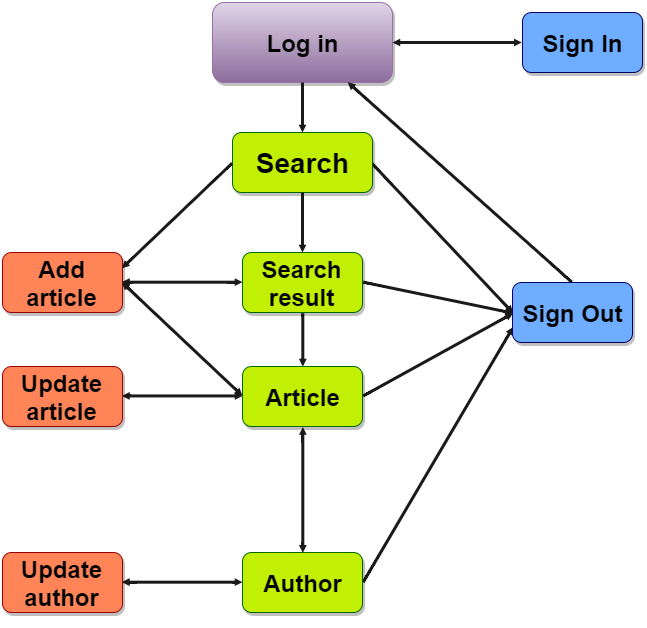
\includegraphics[height=11cm]{sitemap.png}
  \caption{Site Map}
\end{figure}

\newpage
\subsection{Snapshots of the Interface}
~
~
\begin{figure}[h!]
  \centering
      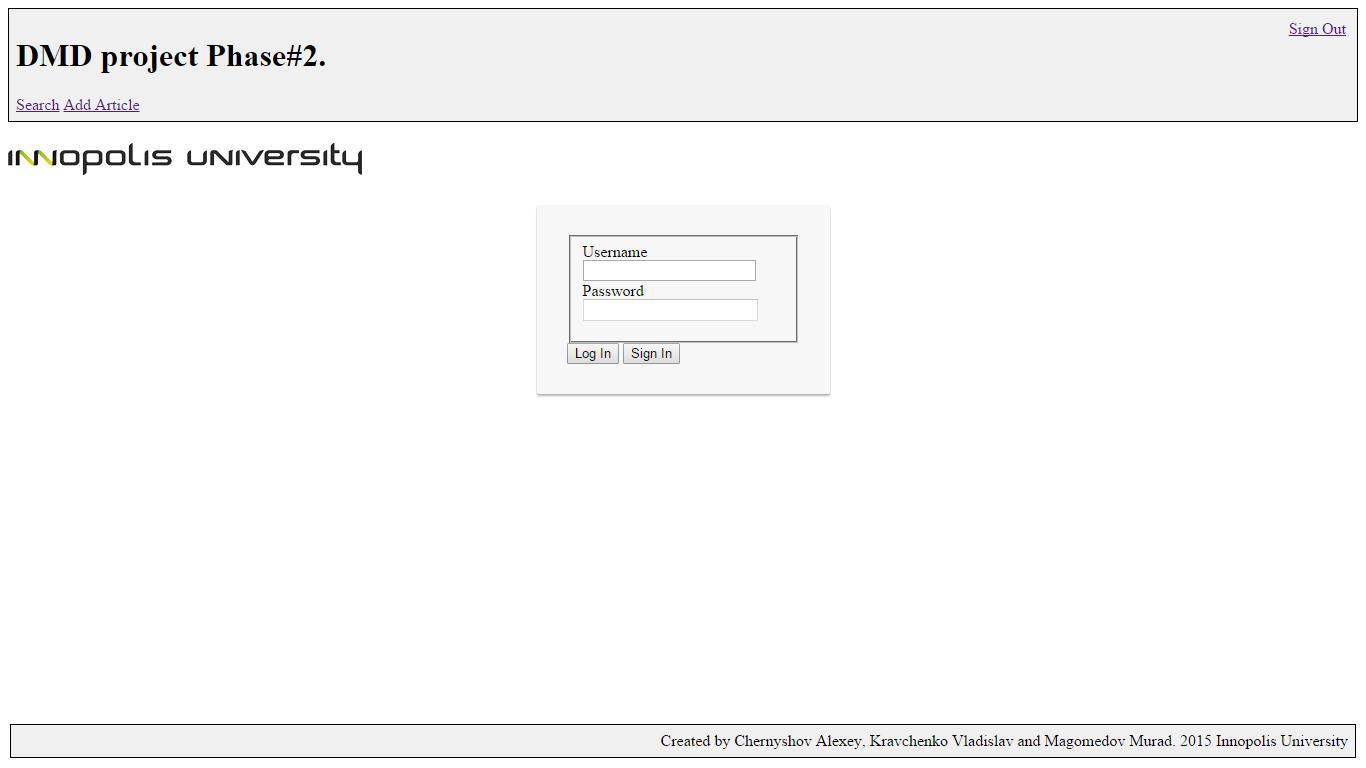
\includegraphics[width=16cm]{1.jpg}
  \caption{Log in or Sign in}
\end{figure}
~
~
\begin{figure}[h!]
  \centering
      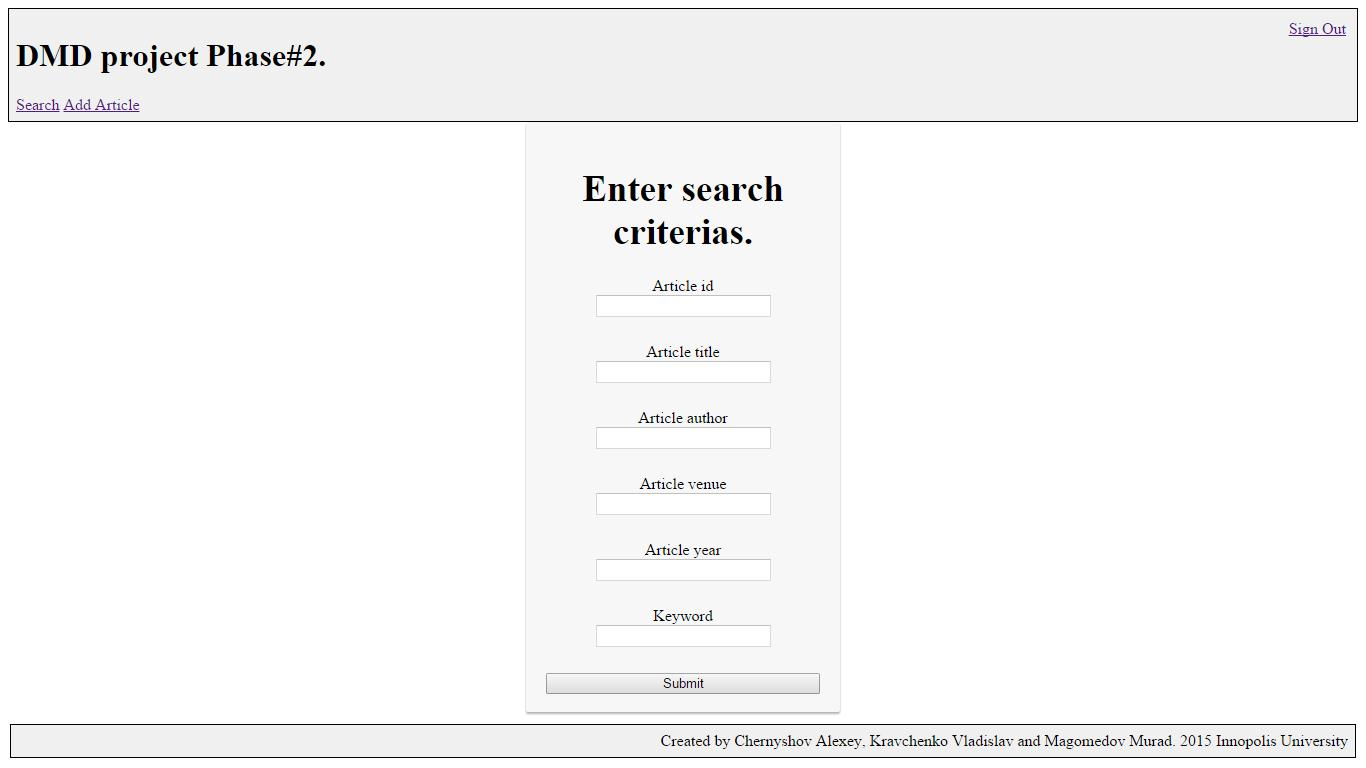
\includegraphics[width=16cm]{2.jpg}
  \caption{Search}
\end{figure}
~
~
\begin{figure}[h!]
  \centering
      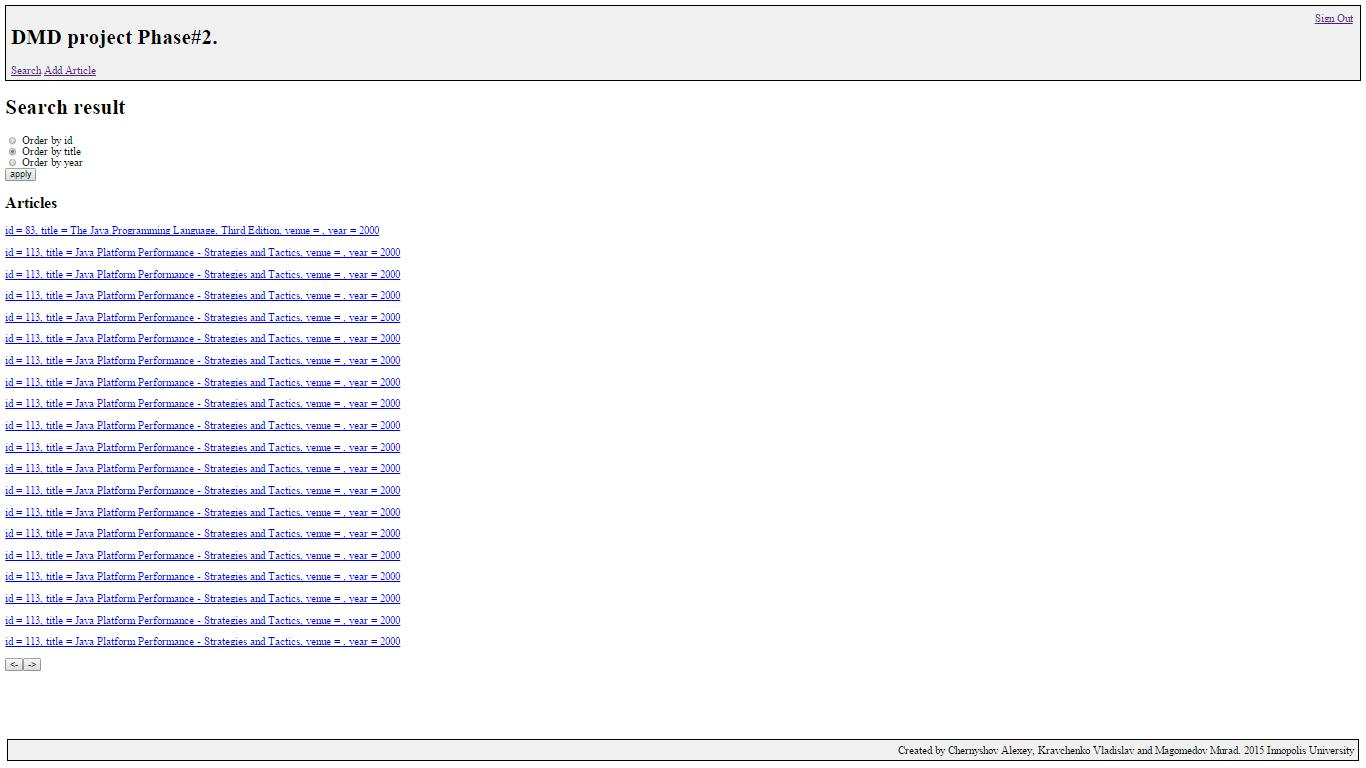
\includegraphics[width=16cm]{3.jpg}
  \caption{Search result}
\end{figure}
~
~
\begin{figure}[h!]
  \centering
      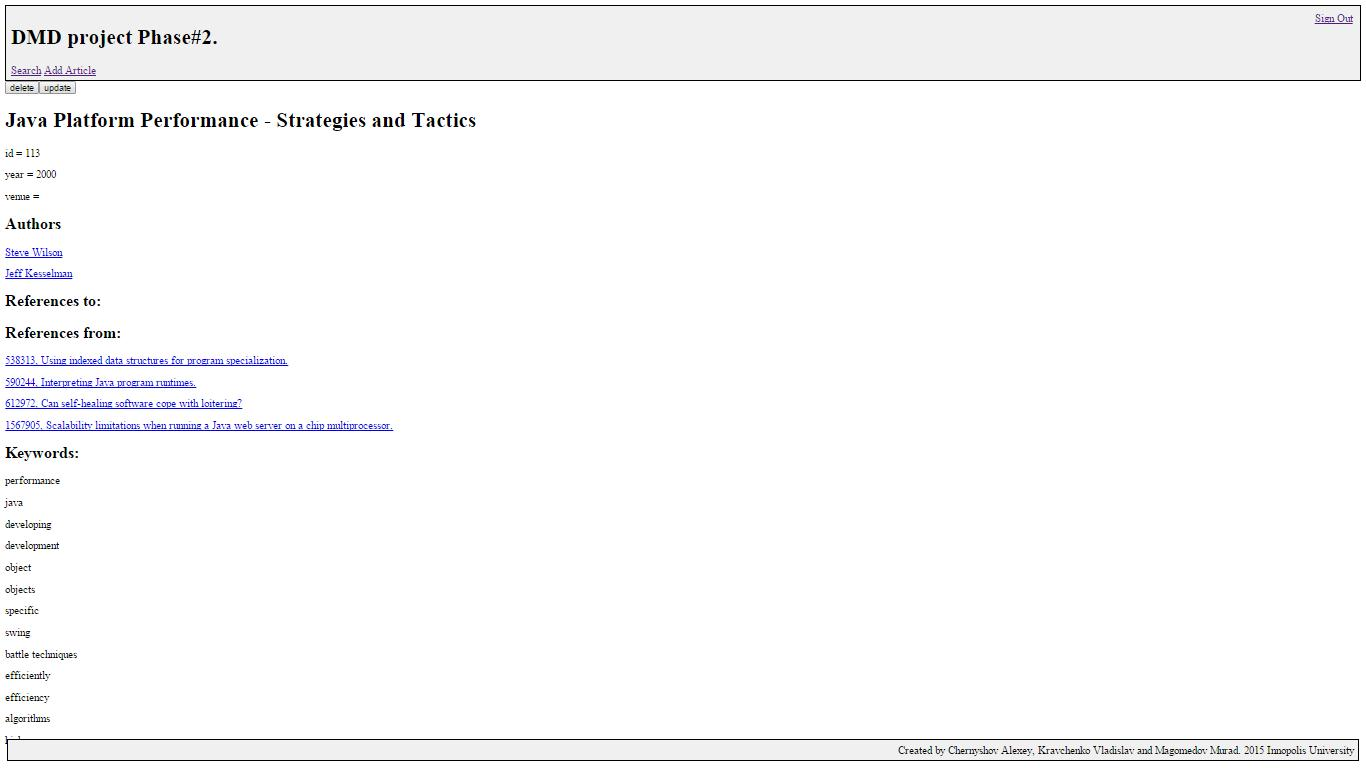
\includegraphics[width=16cm]{4.jpg}
  \caption{Article}
\end{figure}

~
\\


\begin{thebibliography}{1}

\bibitem{def_dblp} 
\url{https://www.python.org/} Python v.3.4

\bibitem{def_tornado} 
\url{http://www.tornadoweb.org} Tornado v.4.2.1

\bibitem{def_tornadobook} 
\ Introduction to Tornado. O’Reilly Media, Inc., 2012. \ ISBN: 978-1-449-30907-7

\bibitem{def_postgresql}
\url{http://www.postgresql.org/} Postgresql v.9.4.5

\bibitem{def_psycopg} 
\url{https://pypi.python.org/pypi/psycopg2} Psycopg2 v.2.6.1


\end{thebibliography}

\end{document}